\documentclass{beamer}

\usepackage[utf8]{inputenc}
\usepackage[english]{babel}

\usepackage{graphicx}
\usepackage{amsmath}
\usepackage{amssymb}
\usepackage{amsthm}
\usepackage{array}

\usepackage{alltt}

\addtocounter{footnote}{1}
\setcounter{tocdepth}{5}
\setcounter{secnumdepth}{5}
\renewcommand{\floatpagefraction}{0.75}

%Information to be included in the title page:
\title{Using textures with OpenGL 3.3}
\author{Alexander Christensen}
\institute{Department of Computer Science \\ University of Copenhagen}
\date{2019}

%% Reference an equation, a figure, or a section

%% \secref{label} - make a reference to a section
\newcommand{\secref}[1]{Section~\ref{#1}}

%% \eqref{reference} - make a reference to an equation
%%\newcommand{\eqref}[1]{(\ref{#1})}

%% \figref{reference} - make a reference to an figure
\newcommand{\figref}[1]{Figure~\ref{#1}}

\newcommand{\basetop}[1]{\vtop{\vskip-1ex\hbox{#1}}}
\newcommand{\source}[1]{\let\thefootnote\relax\footnotetext{\scriptsize\textcolor{kugray1}{Source: #1}}}

%\bibliographystyle{longalpha}
%\bibliography{refs}

%% -*- Mode: latex -*-

%% Macros defined during a long time and used much
% plus - a plus sign
\newcommand{\plus}{+}

% minus - a minus having the same width as a plus
\newlength{\minuswidth}
\settowidth{\minuswidth}{+}
\newlength{\minusheight}
\settoheight{\minusheight}{+}
\newcommand{\minus}{\rule[0.5\minusheight]{\minuswidth}{0.5pt}}

% The basis vector standard
%\renewcommand{\vec}[1]{\boldsymbol{#1}}
\newcommand{\grad}{\operatorname{\nabla}}
\newcommand{\curl}{\operatorname{\text{curl}}}
\newcommand{\divergence}{\operatorname{\text{div}}}
\newcommand{\vecop}{\operatorname{\text{vec}}}
\newcommand{\diag}{\operatorname{\text{diag}}}
\renewcommand{\Re}{\mathbb{R}}
\newcommand{\Co}{\mathbb{C}}
\newcommand{\In}{\mathbb{Z}}
\newcommand{\sign}{\operatorname{sgn}}
%\newcommand{\trace}{\operatorname{Tr}}
\newcommand{\arctantwo}{\ensuremath{\arctan\!2}}
%\newcommand{\mat}[1]{\ensuremath{\boldsymbol{#1} }}
\newcommand{\I}{\mat{1}}
\newcommand{\crossmat}[1]{\ensuremath{\boldsymbol{#1}^{\times} }}
\newcommand{\jacobian}[1]{\ensuremath{\boldsymbol{\mathit{#1}} }}
\newcommand{\set}[1]{\ensuremath{ \boldsymbol{#1} }}
\newcommand{\func}[1]{{\bf{#1}}}
\newcommand{\enorm}[1]{\ensuremath{\left\| #1 \right\|_{_2}}}
%\newcommand{\norm}[1]{\ensuremath{\left\| #1 \right\|}}
\newcommand{\bdet}[1]{\ensuremath{\left| #1 \right|}}
\newcommand{\abs}[1]{\ensuremath{\left| #1 \right|}}
\newcommand{\rtm}{$^{\textrm{®}}$}


\newcommand{\kenny}[1]{ #1 }
\newcommand{\henrik}[1]{ #1 }


%% \maya - the maya signature
\newcommand{\maya}{$ \texttt{Maya}^{\text{\texttrademark}} $}

%% \fat{symbol} - make this symbol fat
\newcommand{\fat}[1]{\mathit{\mathbf{#1}}}
%% \newcommand{\fat}[1]{\hbox{\boldmath $ #1 $}}

%% \vec{symbol} - Vector
%% \renewcommand{\vec}[1]{\mathbf{#1}}
\renewcommand{\vec}[1]{\fat{#1}}

%% \mat{symbol} - Matrix
%%\newcommand{\mat}[1]{\ensuremath{\boldsymbol{#1} }}
\newcommand{\mat}[1]{\fat{#1}}

%% \ezero,...,\ethree - the spin matrices
\newcommand{\ezero}{\begin{bmatrix} 1 & 0 \\  0 &  1 \end{bmatrix}}
\newcommand{\eone}{\begin{bmatrix} i & 0 \\  0 & -i \end{bmatrix}}
\newcommand{\etwo}{\begin{bmatrix} 0 & 1 \\ -1 &  0 \end{bmatrix}}
\newcommand{\ethree}{\begin{bmatrix} 0 & i \\  i &  0 \end{bmatrix}}

%% \quat{symbol} - Quaternion
%% \newcommand{\quat}[1]{\mathbf{#1}}
\newcommand{\quat}[1]{\fat{#1}}

%% \real{quaternion} - the real (scalar) part of a quaternion
\newcommand{\real}{\operatorname{real}}

%% \pure{quaternion} - the pure (vector) part of a quaternion
\newcommand{\pure}{\operatorname{pure}}

%% \sgn{symbol} - the sign of a symbol
\newcommand{\sgn}{\operatorname{sgn}}

%% \norm{symbol} - Norm of a vector/quaternion
\newcommand{\norm}[1]{\parallel {#1} \parallel}

%% \trace{matrix}
\newcommand{\trace}[1]{\mathrm{trace}(#1)}

% This is for code-snippets in the text.
\usepackage{fancyvrb}   %% Try to comment this out if problems with pdflatex
\newcommand{\code}[1]%
%{ \VerbatimInput[frame=none,fontsize=\footnotesize,numbers=none,label=\texttt{#1}]{#1}  }
{ \VerbatimInput[frame=single,fontsize=\footnotesize,numbers=left,label=\texttt{#1}]{#1}  }


%\newcommand{\todo}[1]{ {\Bf Todo:} #1}
\newcommand{\todo}[1]{ }

%\newcommand{\longversion}[1]{ #1 }
\newcommand{\longversion}[1]{ }


\mode<presentation>
{
  \usetheme{Diku}
  \beamertemplatenavigationsymbolsempty
  \setbeamercovered{invisible}
%  \setbeamercovered{transparent=15}
}

%% Kennys pseudocode environment

\newenvironment{pseudocode}{
  \begin{center}
    \begin{minipage}[t]{0.8\columnwidth}
      \footnotesize
      \rule{\columnwidth}{1pt}
    }{
      \rule{\columnwidth}{1pt}
    \end{minipage}
  \end{center}
}

{
\AtBeginSection[wef]
{
\begin{frame}
\frametitle{Table of Contents}
\tableofcontents[currentsection]{1}
\end{frame}
}
}


\begin{document}

% Set background to front page
\usebackgroundtemplate{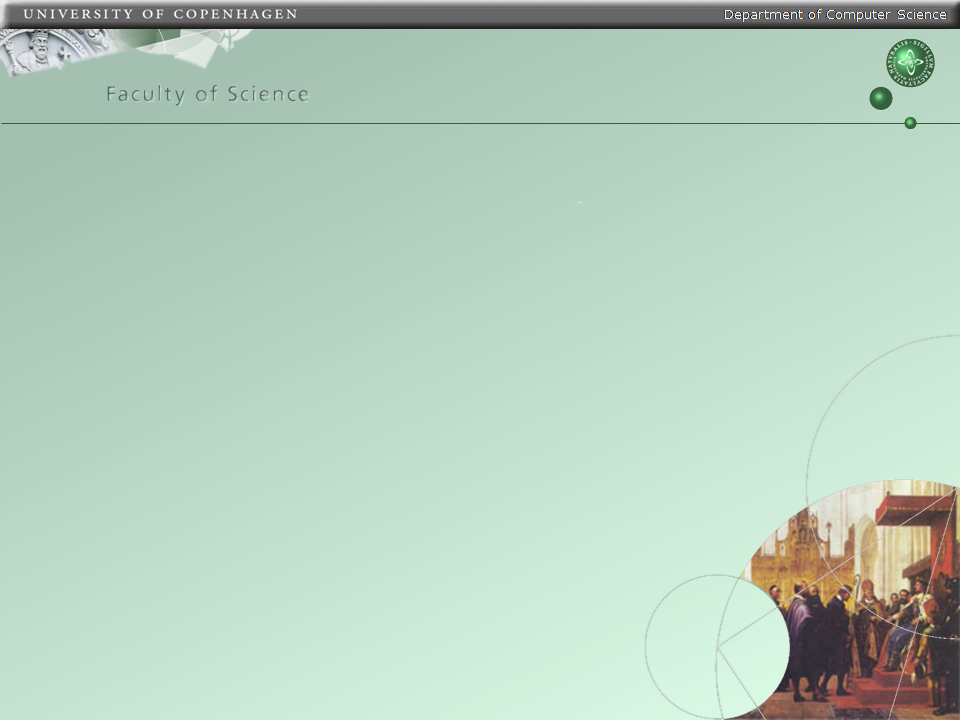
\includegraphics[width=\paperwidth,height=\paperheight]{front}}
{
\begin{frame}[plain]
  \titlepage
\end{frame}
}

% Set background to rest of pages
\usebackgroundtemplate{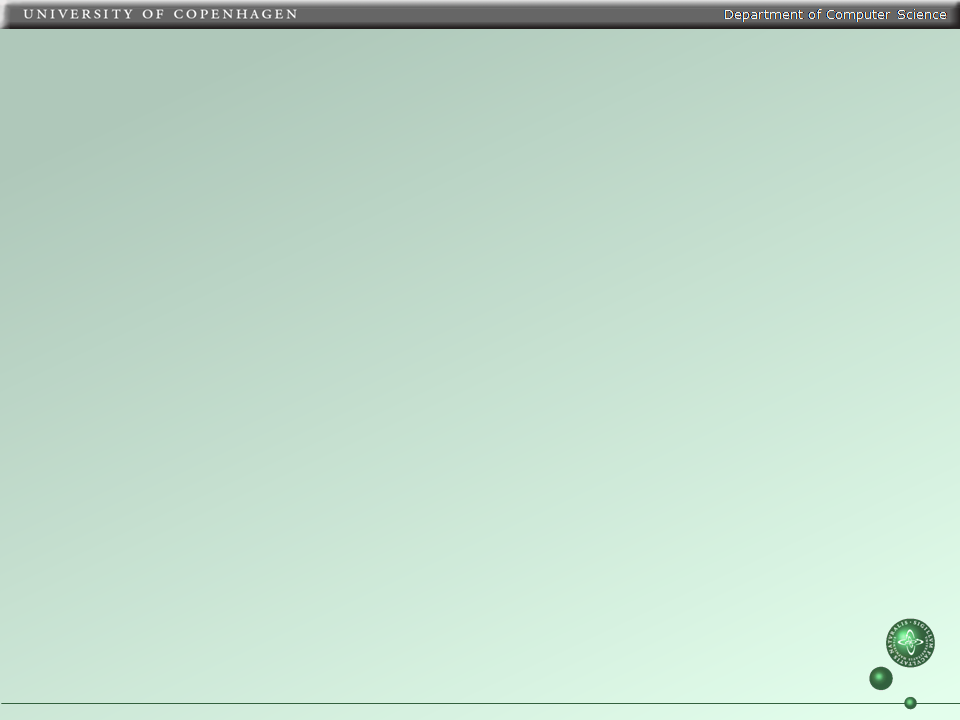
\includegraphics[width=\paperwidth,height=\paperheight]{background}}

%
%
%
\begin{frame}
\frametitle{Overview}
\tableofcontents
%% This is a text in first frame. This is a text in first frame. This is a text in first frame.
\end{frame}


%
%
%
\section{What is a texture?}

\section{Texture Coordinates}

\section{Setting Parameters}

\section{Texture Mapping}

\section{Finding a texture loader}


\begin{frame}
\frametitle{Texture Coordinates}
We define a normalized coordinate system $T : \mathbb{R}^2$.
A coordinate in a texture is called a \textit{texel}, and is a discrete value.
To get a texel given real coordinates $(u,v)$ we can apply a filtering
function $f(u,v)\ :\ \mathbb{R}^2 \mapsto \mathbb{N}^2$.
\begin{figure}
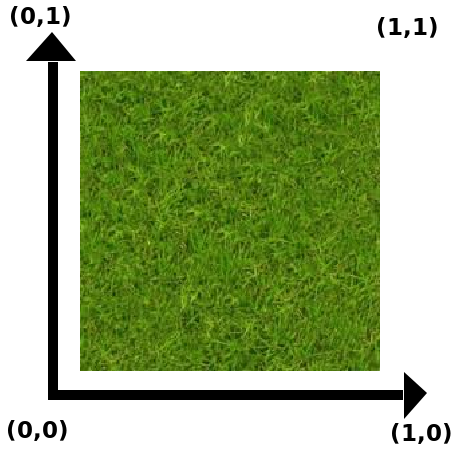
\includegraphics[width=0.5\textwidth]{images/textureCoordinates.png}
\end{figure}
\end{frame}


\begin{frame}
\frametitle{Texture Coordinates - Filtering}
\begin{figure}
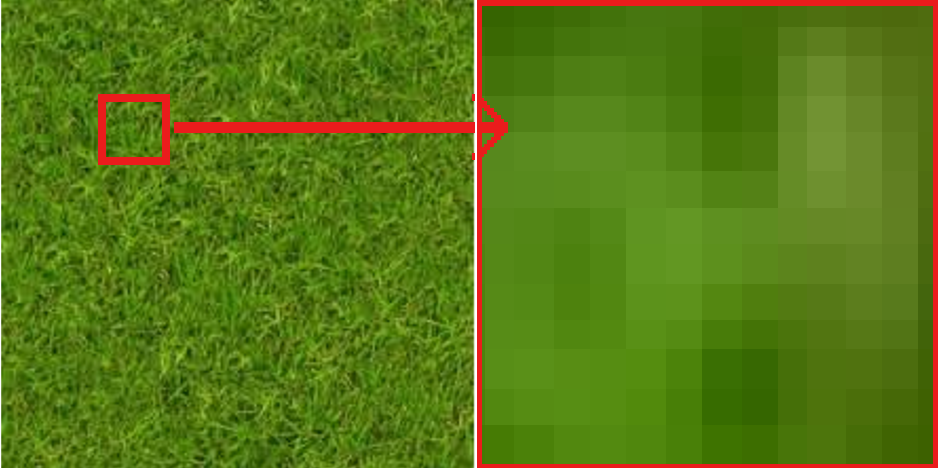
\includegraphics[width=0.7\textwidth]{images/filtering.png}
\caption{filtering}
\end{figure}

Define a function for interpolating between texture coordinates:
\texttt{GL\_NEAREST :} choose nearest texel.\\
\texttt{GL\_LINEAR\ \  :} linearly interpolate over neibhbouring texels.



\end{frame}

\begin{frame}
\frametitle{Setting parameters - Wrapping}
\end{frame}

\begin{frame}
\frametitle{Setting parameters - Clamping}
\end{frame}

\begin{frame}
\frametitle{Setting parameters - Mipmapping}
\end{frame}

\begin{frame}
\frametitle{columns}
\begin{columns}
\column{0.5\textwidth}
Some item on column 1

\column{0.5\textwidth}
Some item on column 2
\end{columns}
\end{frame}


%
%
%
\begin{frame}
\frametitle{Summary}
Text 1

\vspace{5mm}
Text 2

\vspace{5mm}
Text 3
\end{frame}


%
%
%
\begin{frame}
\frametitle{References}
\nocite{*}
\bibliography{refs}{}
\bibliographystyle{alpha}
\end{frame}



\end{document}
